\section{Problem setup}
\label{sec:model}

\begin{figure}[t]
  \begin{centering}
  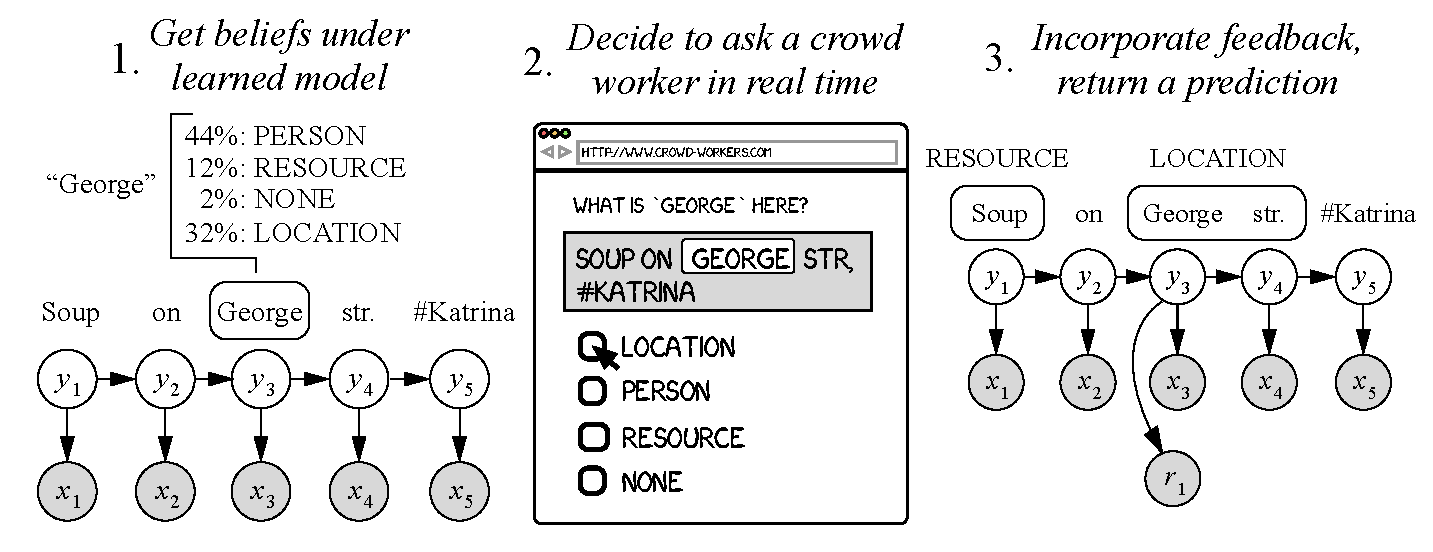
\includegraphics[width=1.0\textwidth]{figures/intro-banner.pdf}
  \end{centering}
  \caption{
    Named entity recognition on tweets in on-the-job training.
    %(1) The system first runs a
%pre-trained model, discovers that the token ``George'' is ambiguous, and then
%asks a human for a label. The human label is returned in a few seconds,
%incorporated into the model, and the model then decides it has enough
%information to turn in a classification.
}
\label{fig:crf}
\end{figure}

\begin{figure}[t]
  \begin{centering}
  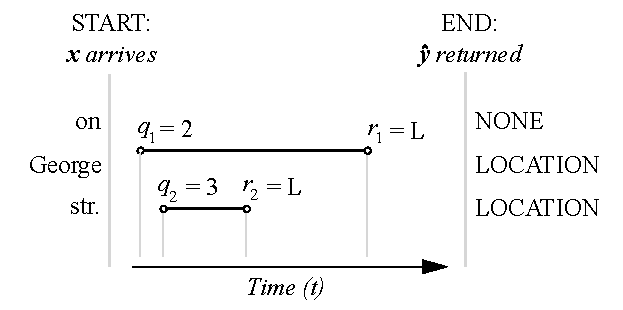
\includegraphics[width=0.56\textwidth]{figures/piano-roll.pdf}
  \hfill
 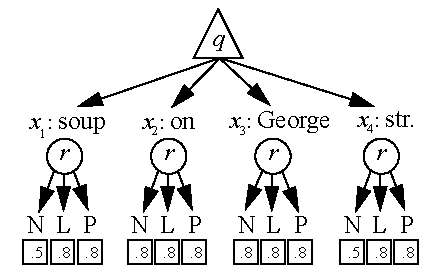
\includegraphics[width=0.43\textwidth,height=0.23\textheight,keepaspectratio]{figures/single-move.pdf}
  \end{centering}
  \caption{
  }
\label{fig:piano-roll}
\end{figure}

% Define structured prediction
Consider a structured prediction problem from input $\bx = (x_1, \dots, x_n)$ to output $\by = (y_1, \dots, y_n)$.
For example, for named-entity recognition on tweets,
$\bx$ is a sequence of words in the tweet (e.g., \nl{on George str.})
and $\by$ is the corresponding sequence of tags (e.g., \scnone{} \scloc{} \scloc{}).
The full set of tags of \scper{}, \scloc{}, \scres{}, and \scnone{}.

% Basic setting
In the \emph{on-the-job training} setting, inputs arrive in a stream.
On each input $\bx$,
we make zero or more queries $q_1, q_2, \dots$ on the crowd to obtain tags
(potentially more than once)
for any positions in $\bx$.
The responses $r_1, r_2, \dots$ come back asynchronously,
which are incorporated into our current prediction model $p_\theta$.
\figureref{piano-roll}(left) shows one possible outcome:
we first query position $q_1 = 2$ (\nl{George}), which later returns $r_1 = \scloc$;
in the meantime, we have queried $q_2=3$ (\nl{str.}) and gotten back $r_2 = \scloc$.
When we have sufficient confidence about the entire output,
we return the most likely prediction $\hat \by$ under the model.
Each query $q_i$ is issued at time $s_i$ and the response comes back at time $t_i$.
Assume that each query costs $m$ cents.
Our goal is to choose queries to maximize accuracy, minimize latency and cost.

% More intuition / connections
We make several remarks about this setting:
First, we must make a prediction $\hat \by$ on each input $\bx$ in the stream,
unlike in active learning, where we are only interested in the pool or stream of examples
for the purposes of building a good model.
% PL: though active learning will query hard examples too
Second, we evaluate on accuracy $\accuracy(\by, \byt)$ against the true tag sequence $\by$
(on named-entity recognition, this is the F$_1$ metric),
but $\by$ is never actually observed---the only feedback is via the responses,
like in partial monitoring games \citep{cesabianchi06regret}.
Therefore, we must make enough queries to garner sufficient confidence
(something we can't do in partial monitoring games)
on each example from the beginning.
Finally, the responses are used to update the prediction model, like in online learning.
This allows the number of queries needed (and thus cost and latency) to decrease over time
without compromising accuracy.

%We receive a stream of inputs $\bx\oft1, \bx\oft2, \ldots, \bx\oft N$ with corresponding {\em unobserved\/} true output $\by\oft1, \by\oft2, \ldots, \by\oft N$ that we would like to predict.

% PL: too much detail about strategy
% at this point, just the get dynamics of the environment set up.
%Let us make our problem setting concrete with an example, depicted in \figureref{piano-roll}.
%We receive an input ``Soup on George str \#Katrina'' ($\bx$) and must produce
%an output ($\byt$) that labels words with the tags.
%Initially, our model is uncertain about both ``George'' and ``str''.
%We first query the crowd for a label on ``George'' ($q_1$) and then for a label on ``str'' ($q_2$). 
%After some time, the crowd responds with the label \scloc{} on both ``George'' ($r_1$) and ``str'' ($r_2$).
%At this point, the model is confident in its labeling, and we can turn in its
%prediction $\byt$.
%By querying the crowd queries $\bq = (q_1, q_2)$, we are not only able to
%produce a more accurate output, but can also use the responses $\br = (r_1,
%r_2)$ to train a better model.

%Of course, querying the crowd also incurs a cost for the queries as well as a
%time delay, $t$: $C(\bq, t)$ \pl{give example numbers that we used}

%In general, we want to maximize our accuracy by making queries while trading
%off the cost and time delay introduced.

% We cast this problem in the Bayesian decision theoretic framework: our objective is to maximize our expected utility under our current model,
% $\p(\by \given \bx, \br)$:
% \begin{align*}
%   u &= \E_{\by \sim \p(\cdot \given \bx, \br)}[1 - \ell(\by, \byt) + C(\bq, t)].
% \end{align*}

%\ac{Probably should talk more about training.} % PL: not really

%We receive a stream of inputs $\bx\oft1, \bx\oft2, \ldots, \bx\oft N$ with corresponding {\em unobserved\/} true output $\by\oft1, \by\oft2, \ldots, \by\oft N$ that we would like to predict.
%For each input $\bx$, we may query the crowd several times. Let $Q = \{q_1, \ldots, q_m\}$ be the set of queries.
%Finally, we observe responses $R = \{r_1, \ldots r_m\}$ to our queries after some time $t$.
%Using the information from these queries, our model makes the prediction, $\byt\oft{t}$.
%Our goal is to maximize the accuracy, trading off cost and latency as specified by a given objective function.
%
%More formally, suppose the output $\by\oft{t}$ has $n$ parts: $\by\oft{t} = y\oft{t}_1, \dots, y\oft{t}_n$.
%Let $q\oft{t} \in \{1, \ldots, n\}$ be a request for the label $y\oft{t}_q$,
%let $Q\oft{t} = (q\oft{t}_1, \dots, q\oft{t}_m)$ be a sequence of queries made on the $t$-th input and
%let $\tau\oft{t}$ be the time taken to make the prediction $\byt\oft{t}$. 
%We would like to minimize the cumulative loss, 
%following objective:
%\begin{align}
%  \sL &= \sum_{t=1}^T \ell_{\rmclass}(\by\oft{t}, \byt\oft{t}) + C(Q\oft{t}, \tau\oft{t}), \label{eqn:objective}
%\end{align}
%where $\ell_{\rmclass}$ is a given misclassification loss function, e.g.\ the Hamming loss, and $C$ is a given cost function.
%\ac{Concern: by using the cumulative loss, is there an expectation that we will ``model'' input and optimize for the future?}
%
%We now describe our choice of models for prediction, human error and latencies and return to optimizing \equationref{objective} in \sectionref{async}.
%
